\documentclass{standalone}
\usepackage{amsmath}
\usepackage{tikz}
\usepackage{enumitem}
\usetikzlibrary{arrows, shapes, calc, backgrounds, fit, decorations.markings, shadows}

\begin{document}

	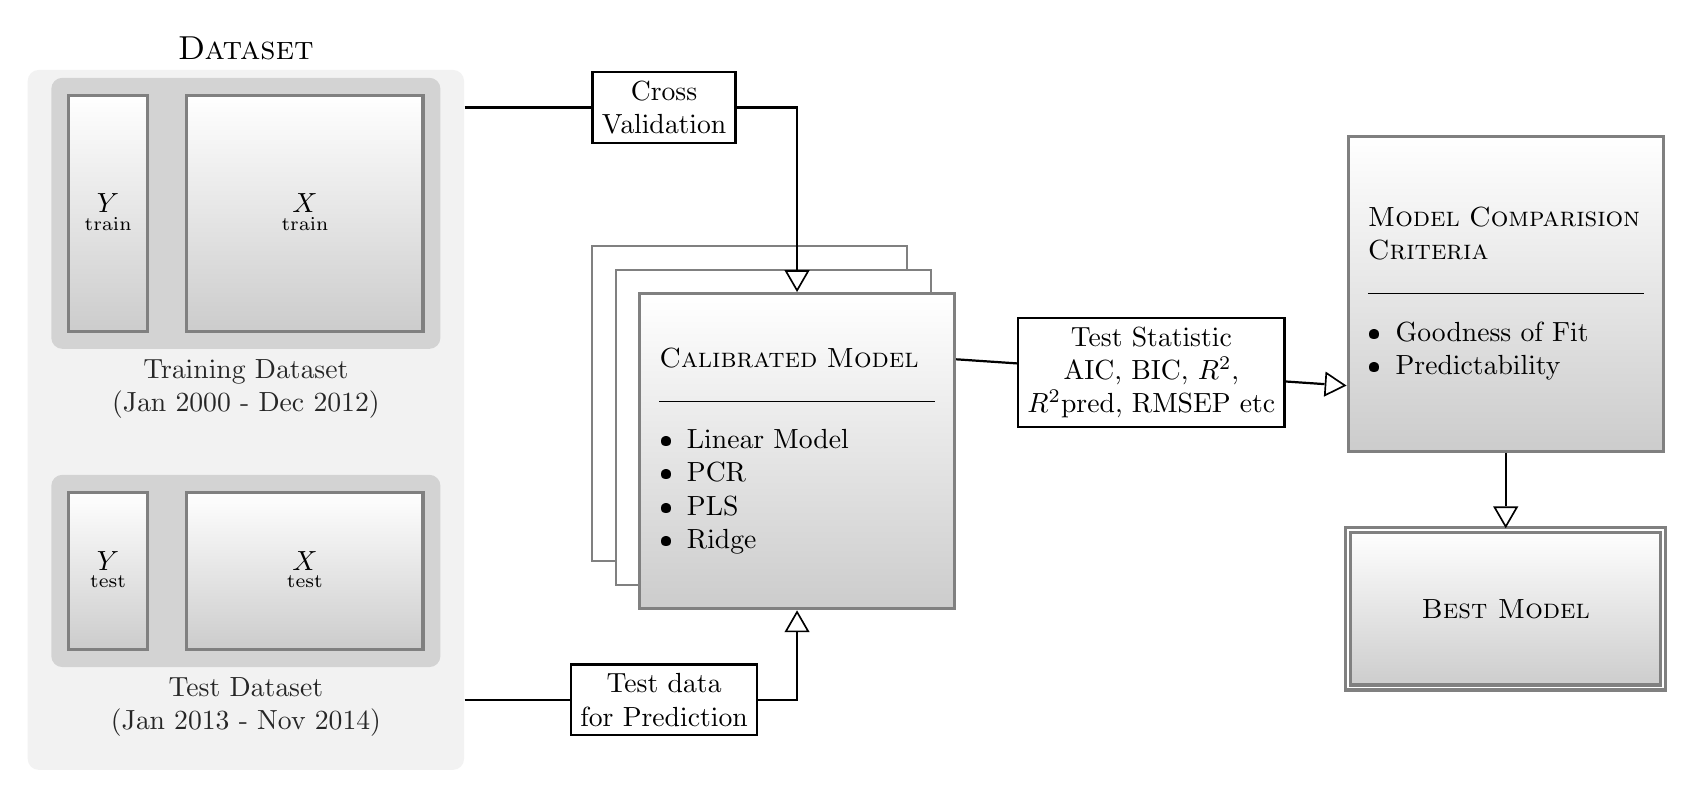
\begin{tikzpicture}[
	every matrix/.style={column sep=3cm,row sep=2cm},
	pblock/.style = {rectangle split, rectangle split parts=2, very thick,draw=black!50, top color=white,bottom color=black!20, align=center, minimum height=3cm},
	block/.style = {rectangle,very thick,draw=black!50, top color=white, bottom color=black!20, align=center, minimum height=#1},
	myarrow/.style = {thick, shorten >= 8pt, decoration={markings,mark=at position 1 with {\arrow[scale=1.5,thin]{open triangle 60}}},
	preaction={decorate}},
	cascaded/.style = {%
	    general shadow = {%
	      shadow scale = 1,
	      shadow xshift = -4ex,
	      shadow yshift = 4ex,
	      draw,
	      thick,
	      fill = white},
	    general shadow = {%
	      shadow scale = 1,
	      shadow xshift = -2ex,
	      shadow yshift = 2ex,
	      draw,
	      thick,
	      fill = white},
	    fill = white, 
	    draw,
	    thick,
	    minimum width = 1.5cm,
	    minimum height = 2cm},                 
	]
	\matrix(dataBlock){
	\node[block={3cm}, minimum width =1cm] (Ytrain) {$\underset{\text{train}}{Y}$};
	\node[block={3cm}, right of = Ytrain, node distance=2.5cm, minimum width=3cm](Xtrain){$\underset{\text{train}}{X}$};\\
	
	\node[block={2cm}, minimum width =1cm, below of=Ytrain] (Ytest) {$\underset{\text{test}}{Y}$};
	\node[block={2cm}, right of = Ytest, node distance=2.5cm, minimum width=3cm, align=center](Xtest){$\underset{\text{test}}{X}$};\\
};
	\begin{scope}[on background layer]
	   \node(trainSet) [fit=(Ytrain) (Xtrain), fill= gray!30, rounded corners, inner sep=.2cm, label={[align=center, name=trainLabel]below:Training Dataset\\(Jan 2000 - Dec 2012)}] {};
	   \node(testSet) [fit=(Ytest) (Xtest), fill= gray!30, rounded corners, inner sep=.2cm, label={[align=center, name=testLabel]below:Test Dataset\\(Jan 2013 - Nov 2014)}] {};
	   	 \begin{scope}[on background layer]
	   	 	\node(dataSet) [fit=(Ytrain) (Xtrain) (Ytest) (Xtest) (trainLabel) (testLabel), fill= gray!50, rounded corners, inner ysep=0.3cm, inner xsep=0.5cm, fill opacity=0.2, label={[yshift=0cm]\large\textsc{Dataset}}] {};
	   	 \end{scope}
	 \end{scope}

	\node[cascaded, block={4cm}, minimum width=4cm, align=center, text width=3.5cm, right of=dataBlock, node distance=7cm, yshift=-1cm](trainedModel){\begin{minipage}{\textwidth}
	\setlist[itemize]{leftmargin=*}
	\textsc{Calibrated Model} \\ \hrule \vfill
		\begin{itemize}[noitemsep]
			\item Linear Model
			\item PCR
			\item PLS
			\item Ridge
		\end{itemize}
	\end{minipage}};
	
	\node[block={4cm}, minimum width=4cm, align=center, text width=3.5cm, right of=trainedModel, node distance=9cm, yshift=2cm](compCriteria){\begin{minipage}{\textwidth}
	\setlist[itemize]{leftmargin=*}
		\textsc{Model Comparision Criteria} \\ \hrule \vfill
		\begin{itemize}[noitemsep]
		\item Goodness of Fit
		\item Predictability
		\end{itemize}
		\end{minipage}};

	\node[double, block={2cm}, minimum width=4cm, below of=compCriteria, node distance=4cm](Final){\textsc{Best Model}};
	
		\draw[myarrow](dataSet.55) -| node[fill=white, rectangle, draw, align=center, pos=0.3]{Cross\\ Validation} (trainedModel.north);
		\draw[myarrow](dataSet.308) -| node[fill=white, rectangle, draw, align=center, pos=0.3]{Test data \\for Prediction} (trainedModel.south);
		\draw[myarrow](trainedModel.30) -- node[fill=white, draw, rectangle, align=center, pos=0.5]{Test Statistic \\AIC, BIC, $R^2$, \\$R^2$pred, RMSEP etc} (compCriteria.210);
		\draw[myarrow](compCriteria) -- (Final);
		
	\end{tikzpicture}
\end{document}